\documentclass{article}
\usepackage[utf8]{inputenc}
\usepackage[spanish]{babel}
\usepackage{listings}
\usepackage{graphicx}
\usepackage{cite}

\begin{document}

\begin{titlepage}
    \begin{center}
        \vspace*{1cm}
            
        \Huge
        \textbf{Informe Parcial 1}
            
        \vspace{0.5cm}
        \LARGE
        Informática II
            
        \vspace{1.5cm}
            
        \textbf{Daniel Perez\\Miguel Serna\\Jorge Montaña}
            
        \vfill
            
        \vspace{0.8cm}
            
        \Large
        Departamento de Ingeniería Electrónica y Telecomunicaciones\\
        Universidad de Antioquia\\
        Medellín\\
        Abril de 2021
            
    \end{center}
\end{titlepage}

\tableofcontents

\section{Análisis del problema}
El primer reto era evidente, debíamos conectar 64 luces LED a la mínima cantidad de pines posibles, claro esta, haciendo uso del dispositivo 74CH595 presentado en la clase, para si poder ampliar la cantidad de salidas digitales.\\

Terminado con eso, podríamos empezar a buscar métodos para encender ciertos LED y dejar los otros apagados y así poder formar figuras con la matriz 8x8, la opción mas lógica sería primero encender todos los LED y poner dicha solución en la función 'Verificación'. A partir de la solución usada en la función 'Imagen', la usaríamos en 'Publik' para que almacene los 3 caracteres deseados e imprima uno por uno.\\

Además de eso, debíamos hacer uso del serial para darle indicaciones al usuario y para que pudiese ingresar el numero, letra o carácter deseado y  aclarar las restricciones en el manual de usuario para así no generar errores.


\section{Algoritmo Implementado} \label{contenido}
\begin{lstlisting}
char texto = "aquí";
\end{lstlisting}
\section{Problemas de desarrollo} \label{conclulsion}
El principal de los problemas que se nos presento fue sobre como íbamos a indicar los valores que los LED debían tener para formar cada letra, al final decidimos realizarlo de la forma mas obvia y lógica, simplemente dando los valores en binario a cada fila para formar dicho carácter, por ejemplo, una fila completamente encendida seria [1,1,1,1,1,1,1,1] y con esa misma lógica podríamos  'dibujar' las matrices fila por fia de cada letra. \\
se nos genero un error de conexión de los LEDs porque se formaban las figuras, pero al revés
\section{Evolución del algoritmo} \label{conclulsion}
\section{Esquema} \label{contenido}
\begin{figure}
    \centering
    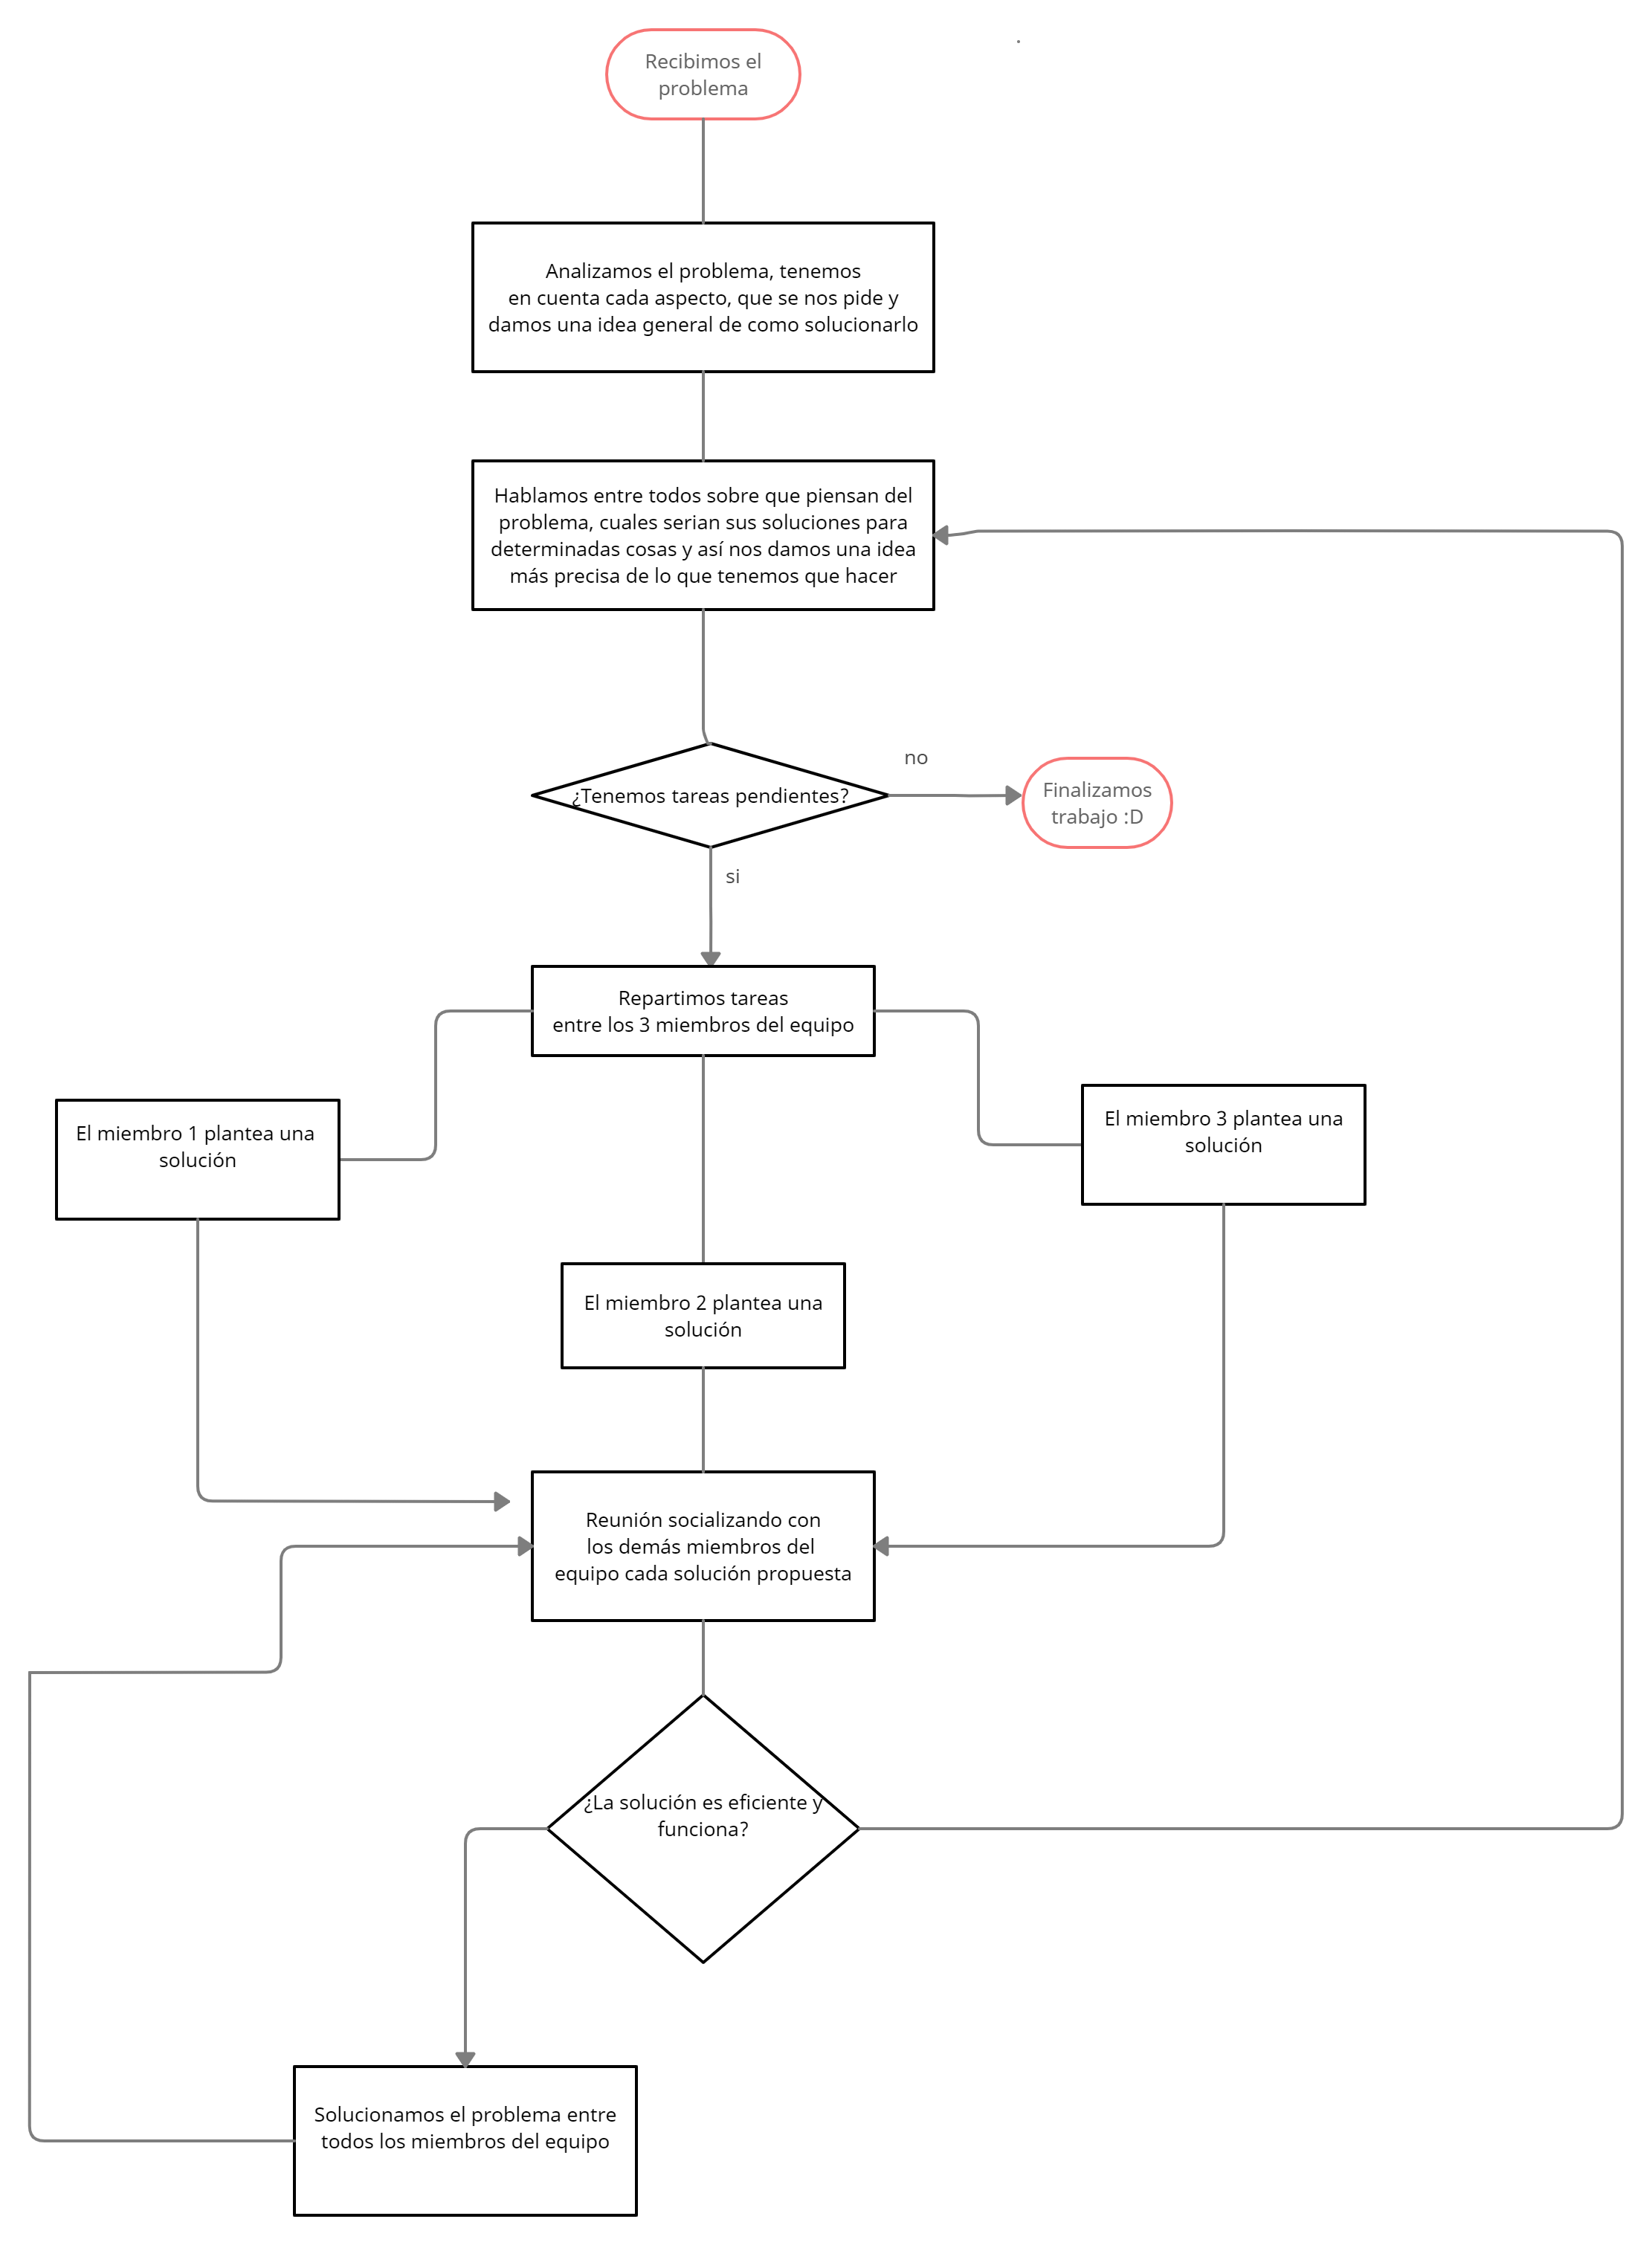
\includegraphics[width=14cm]{diagrama.png}
    \caption{diagrama}
    \label{fig:my_label}
\end{figure}
\bibliographystyle{IEEEtran}
\bibliography{references}

\end{document}